In this section we document the kinematic distributions in the 
Top background enriched regions. We apply the same selections as in the 
WW preselection except that we invert the top veto requirements. 

%%%%%%%%%%%%%%%%%%%%%%%%%%%%%%%%%%%%
\begin{figure}[!hbtp]
\centering
\subfigure[Leading lepton $p_T$]{
\centering
\label{subfig:ptmax}
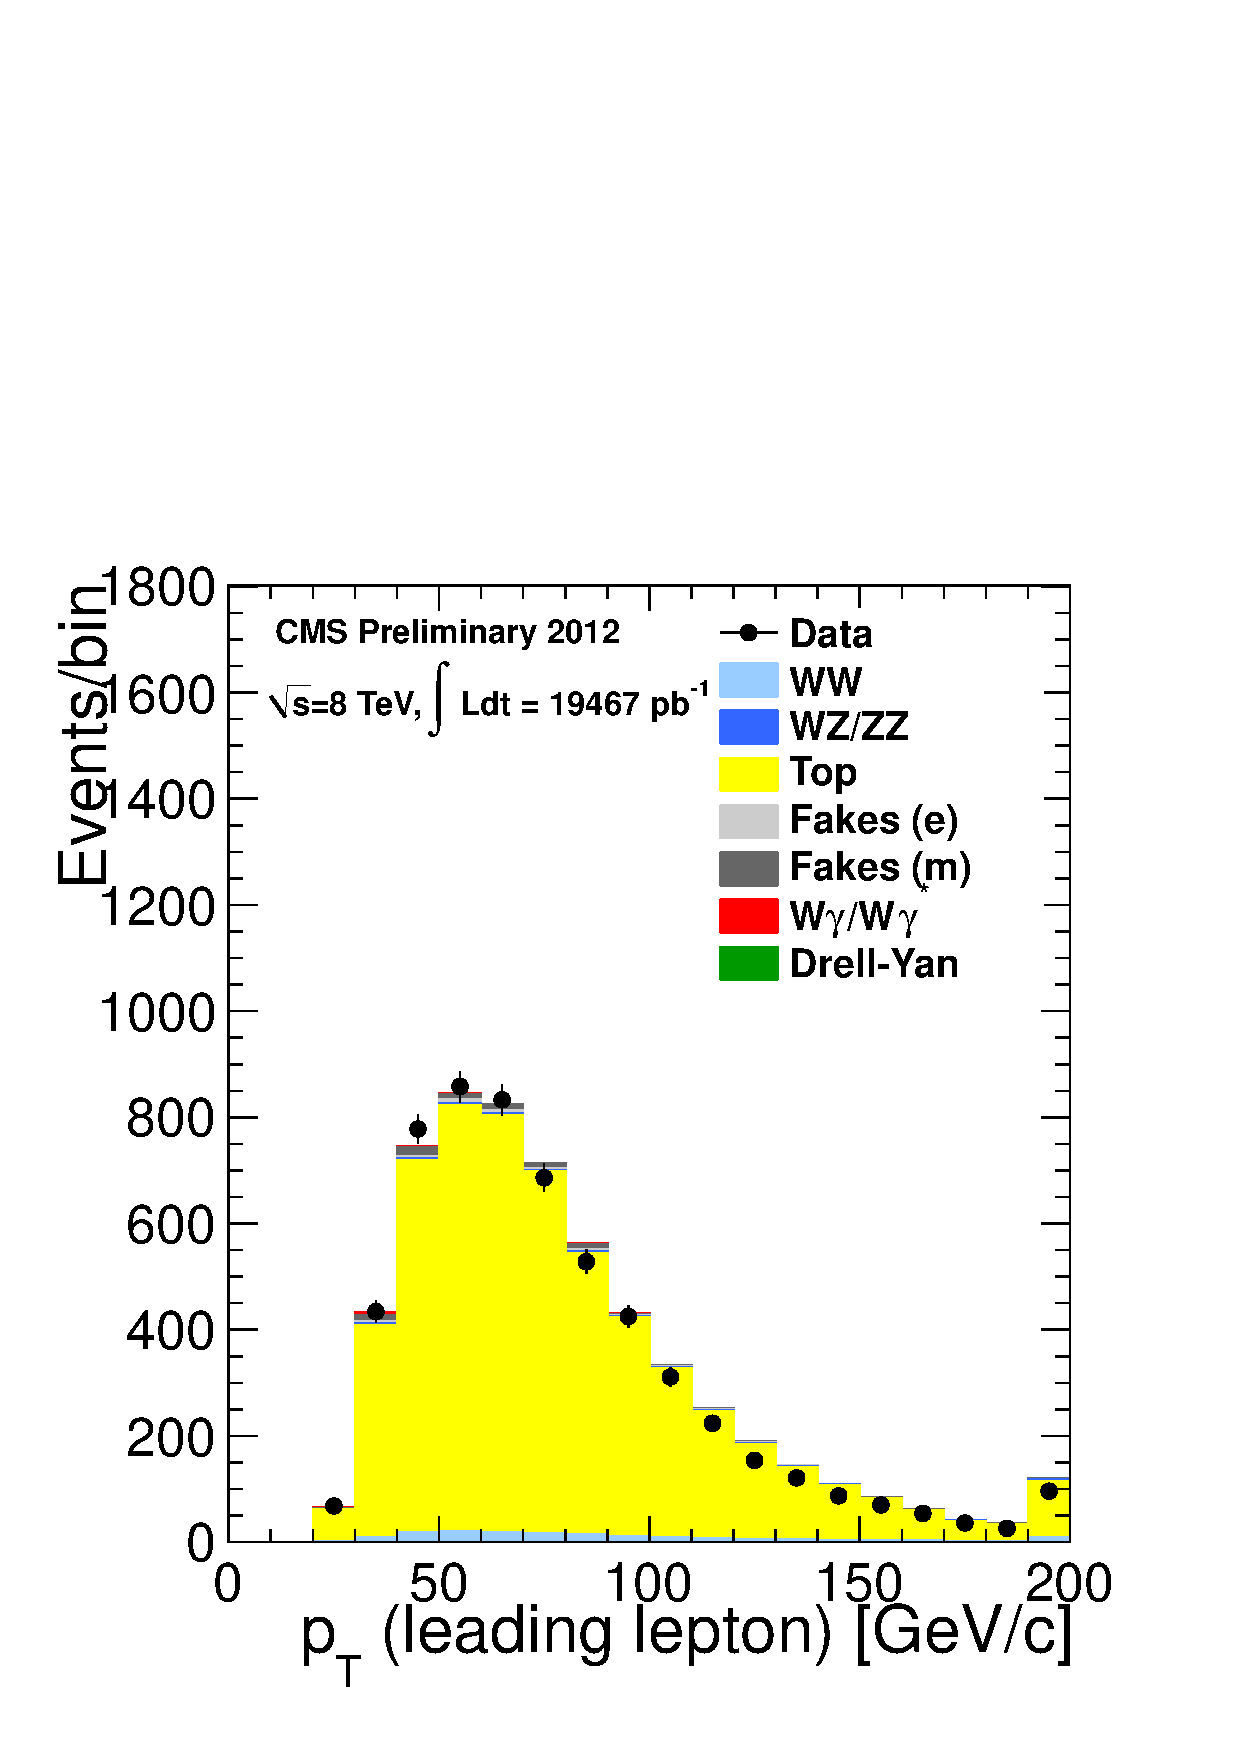
\includegraphics[width=.31\textwidth]{figures/hww_analysis16_0_ALL_of_1j_pt1_toptag.pdf}
}
\subfigure[Trailing lepton $p_T$]{
\centering
\label{subfig:ptmin}
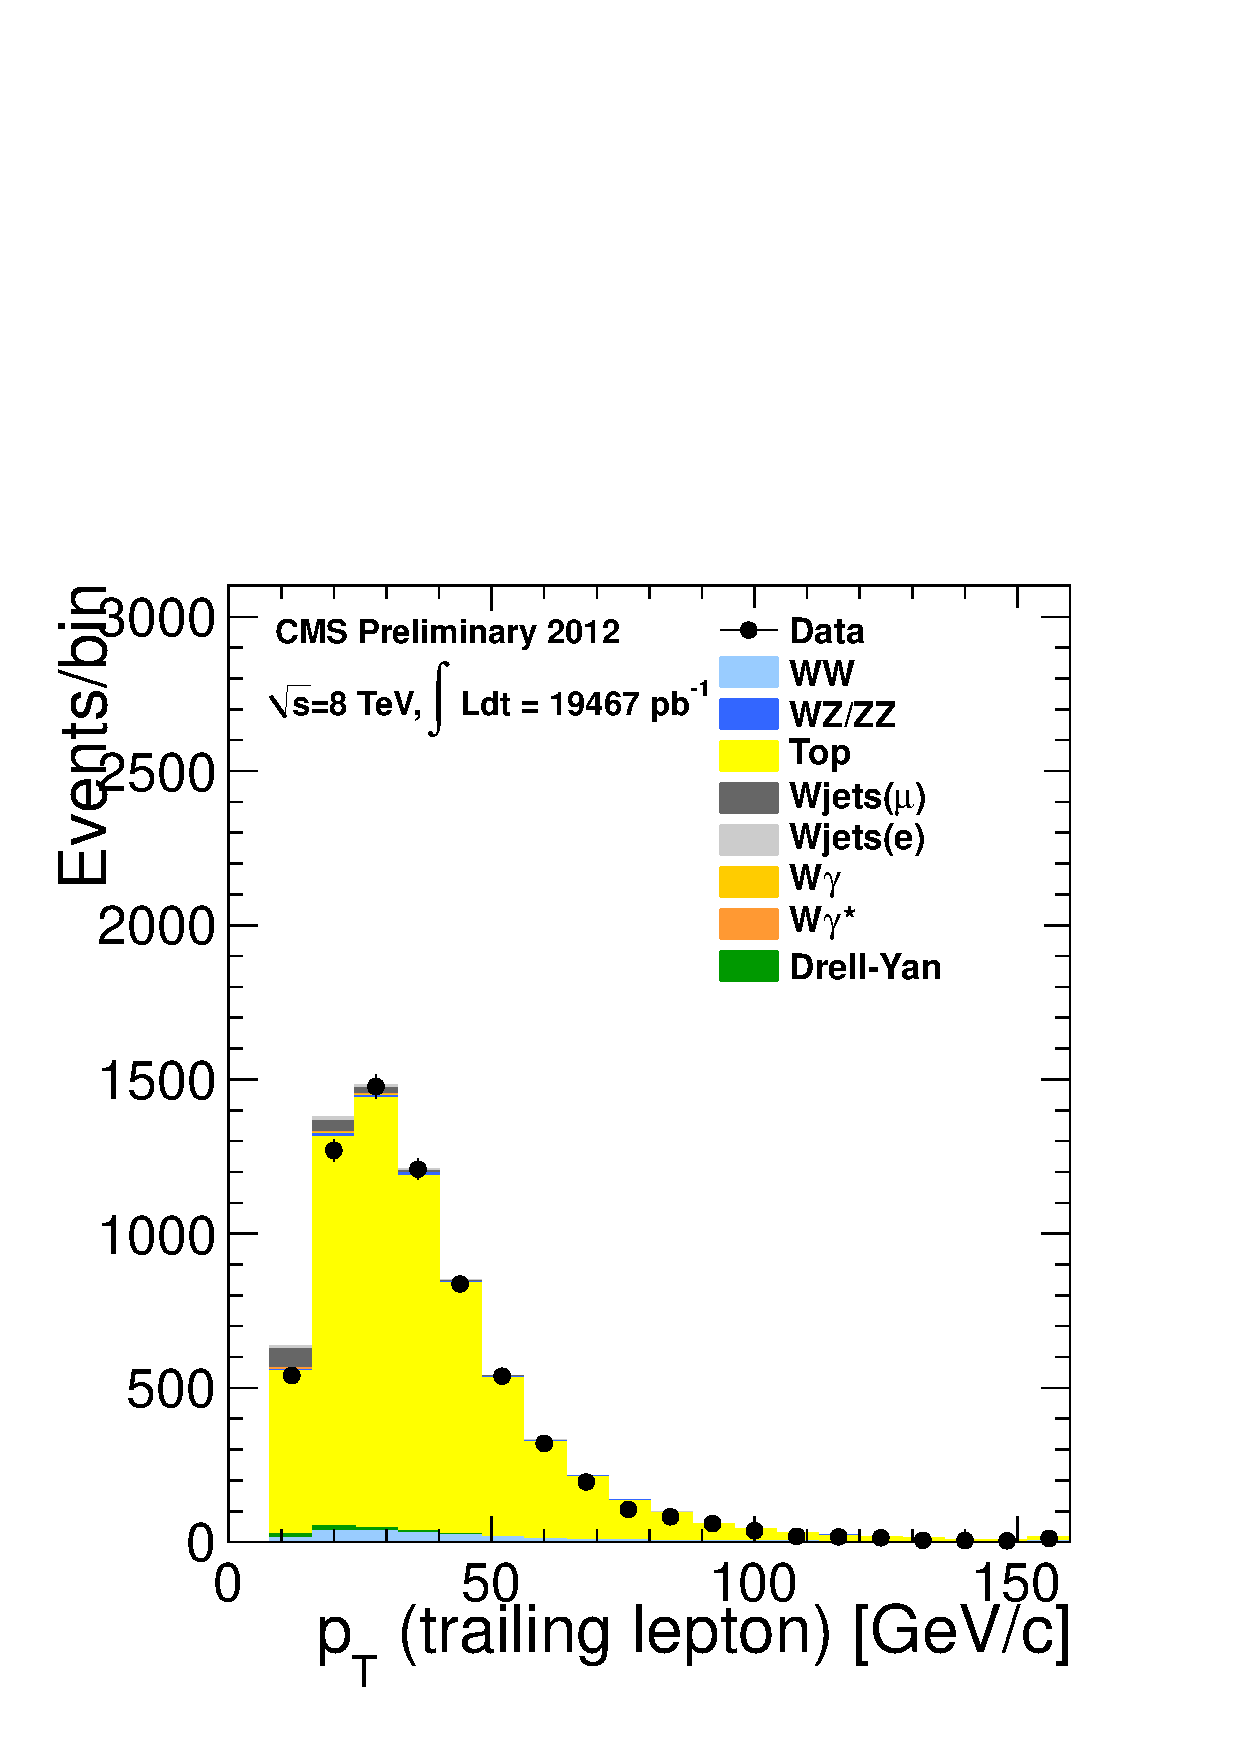
\includegraphics[width=.31\textwidth]{figures/hww_analysis16_0_ALL_of_1j_pt2_toptag.pdf}
}
\subfigure[Dilepton mass]{
\centering
\label{subfig:mll}
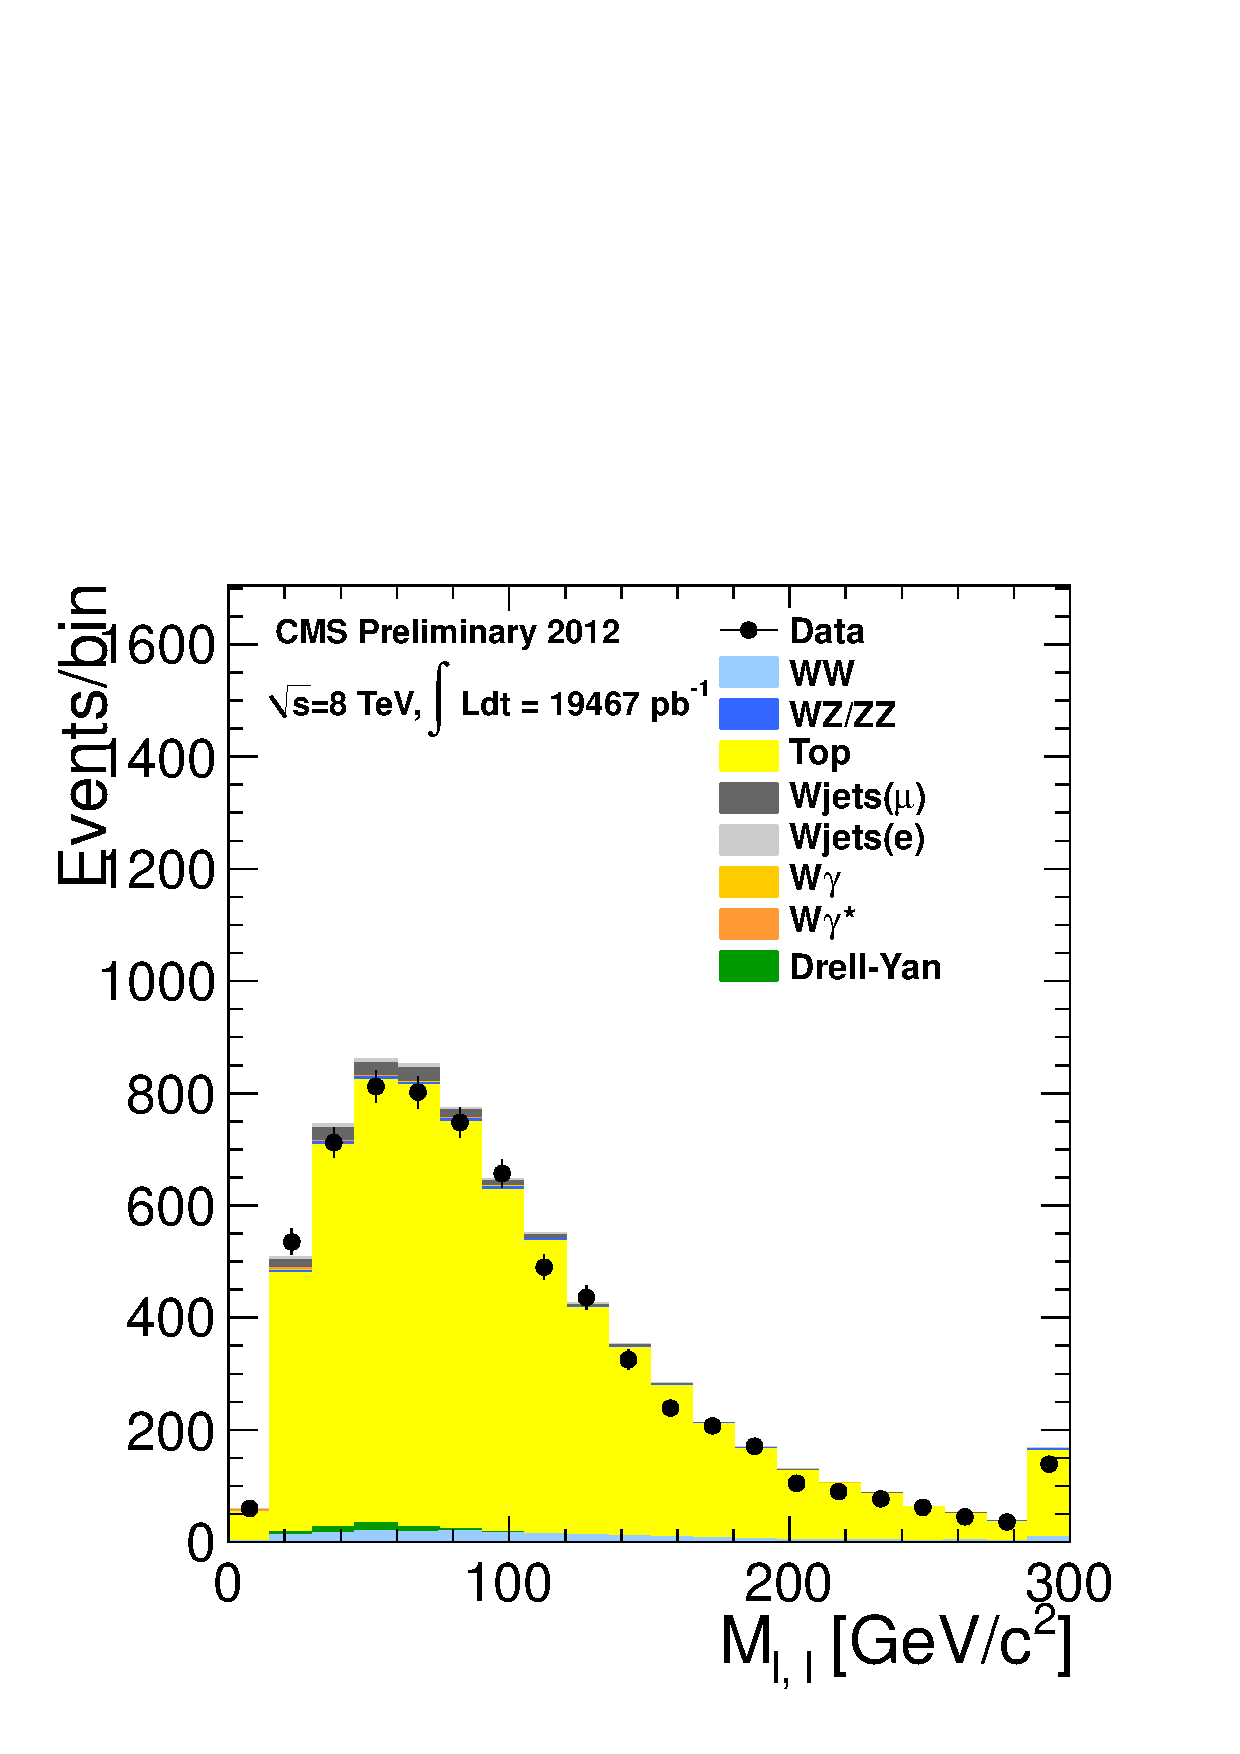
\includegraphics[width=.31\textwidth]{figures/hww_analysis16_0_ALL_of_1j_mll_toptag.pdf}
} \\
\subfigure[$\Delta\phi(\ell,\ell)$]{
\centering
\label{subfig:dphi}
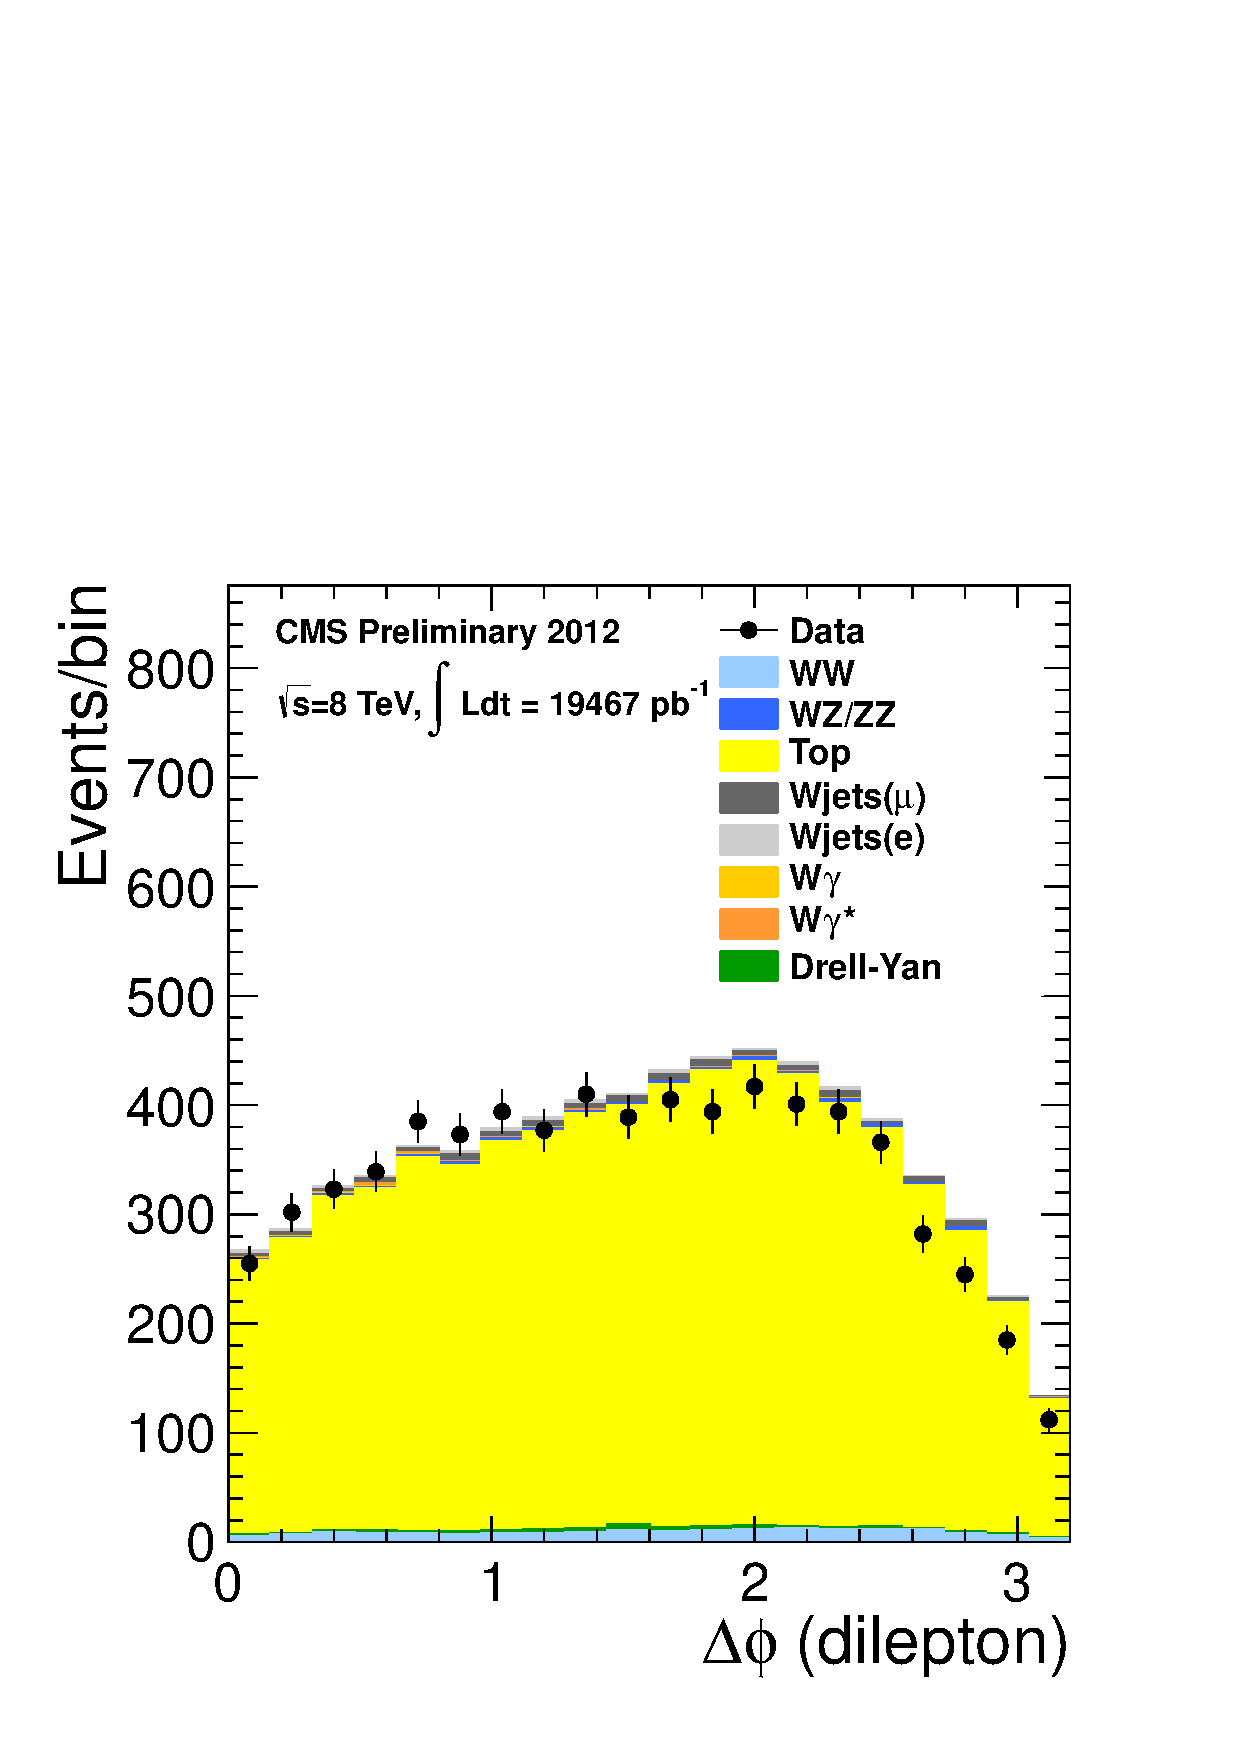
\includegraphics[width=.31\textwidth]{figures/hww_analysis16_0_ALL_of_1j_dphi_toptag.pdf}
}
\subfigure[MET]{
\centering
\label{subfig:ptmax}
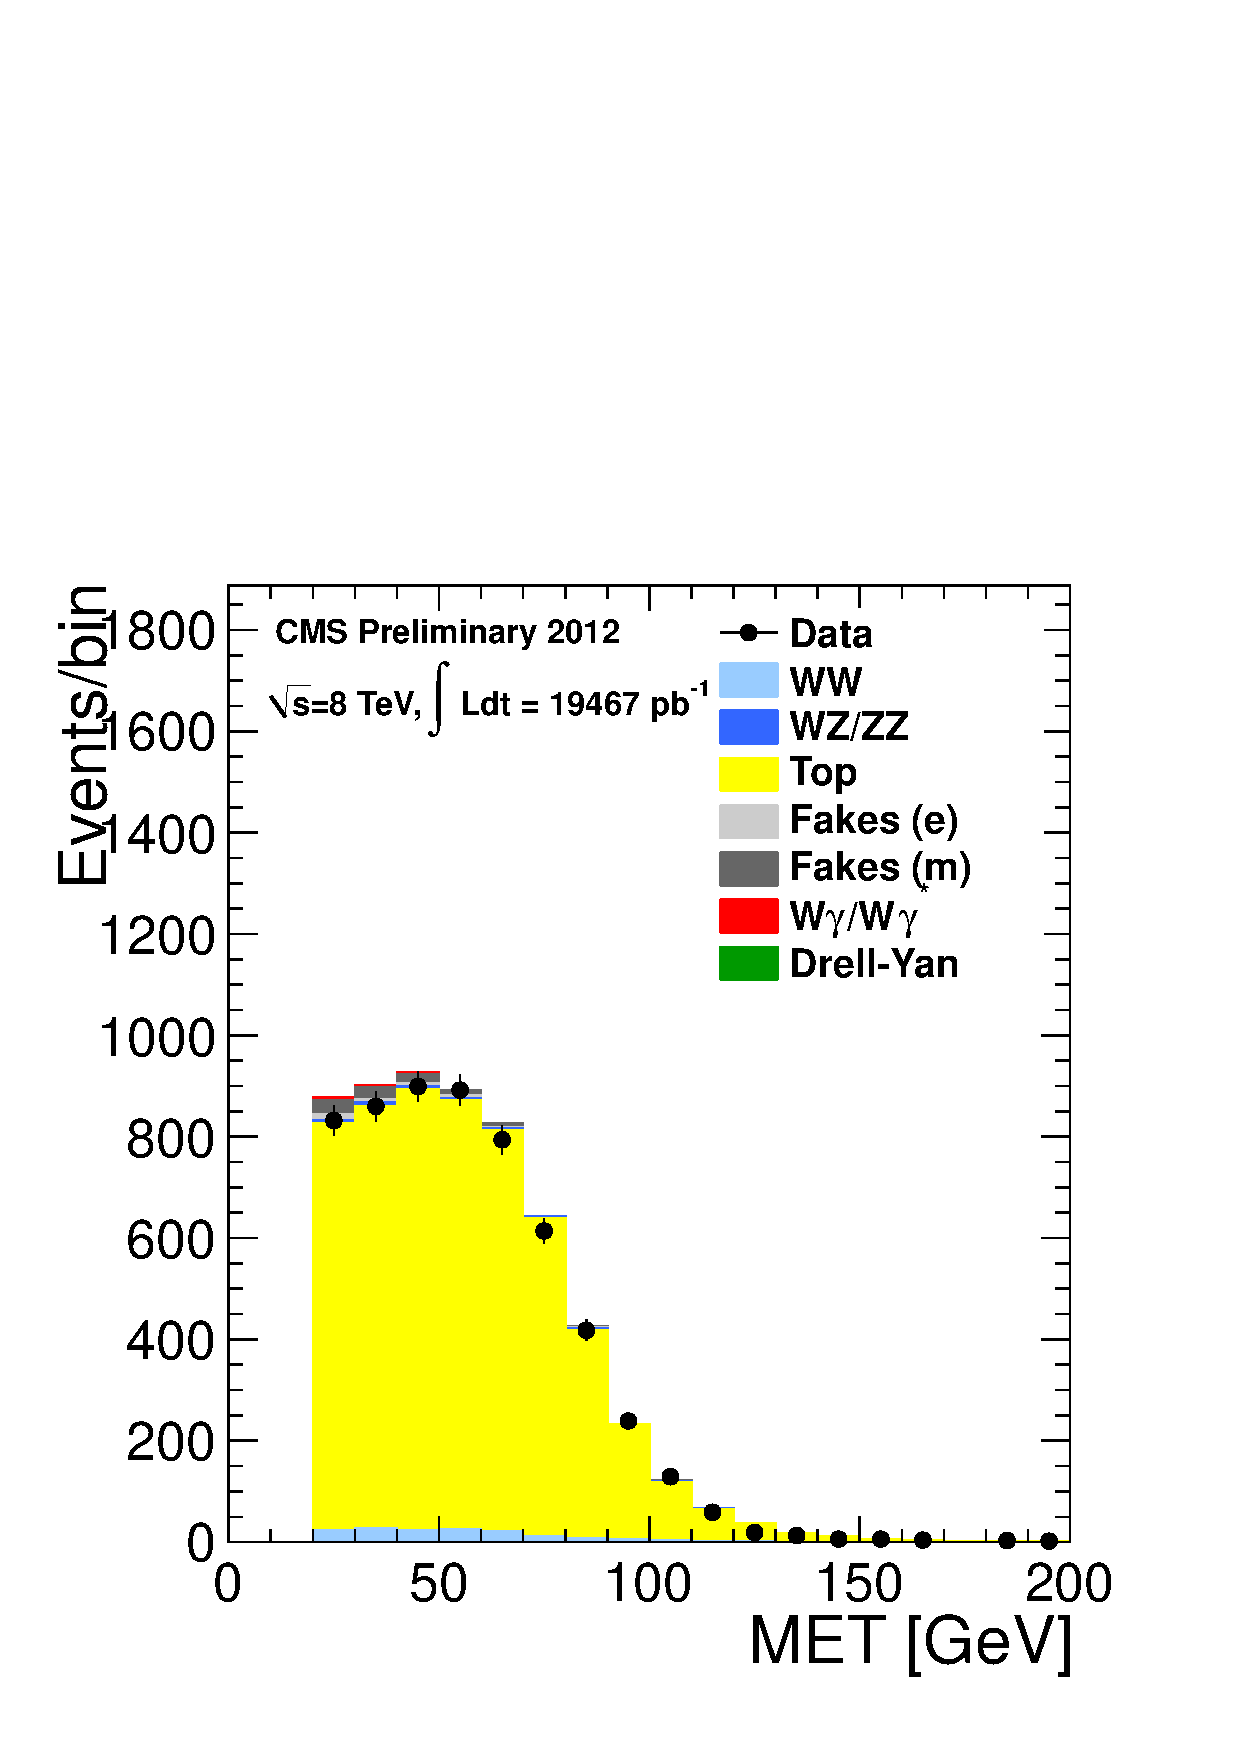
\includegraphics[width=.31\textwidth]{figures/hww_analysis16_0_ALL_of_1j_met_toptag.pdf}
}
\subfigure[Transverse Higgs Mass]{
\centering
\label{subfig:ptmin}
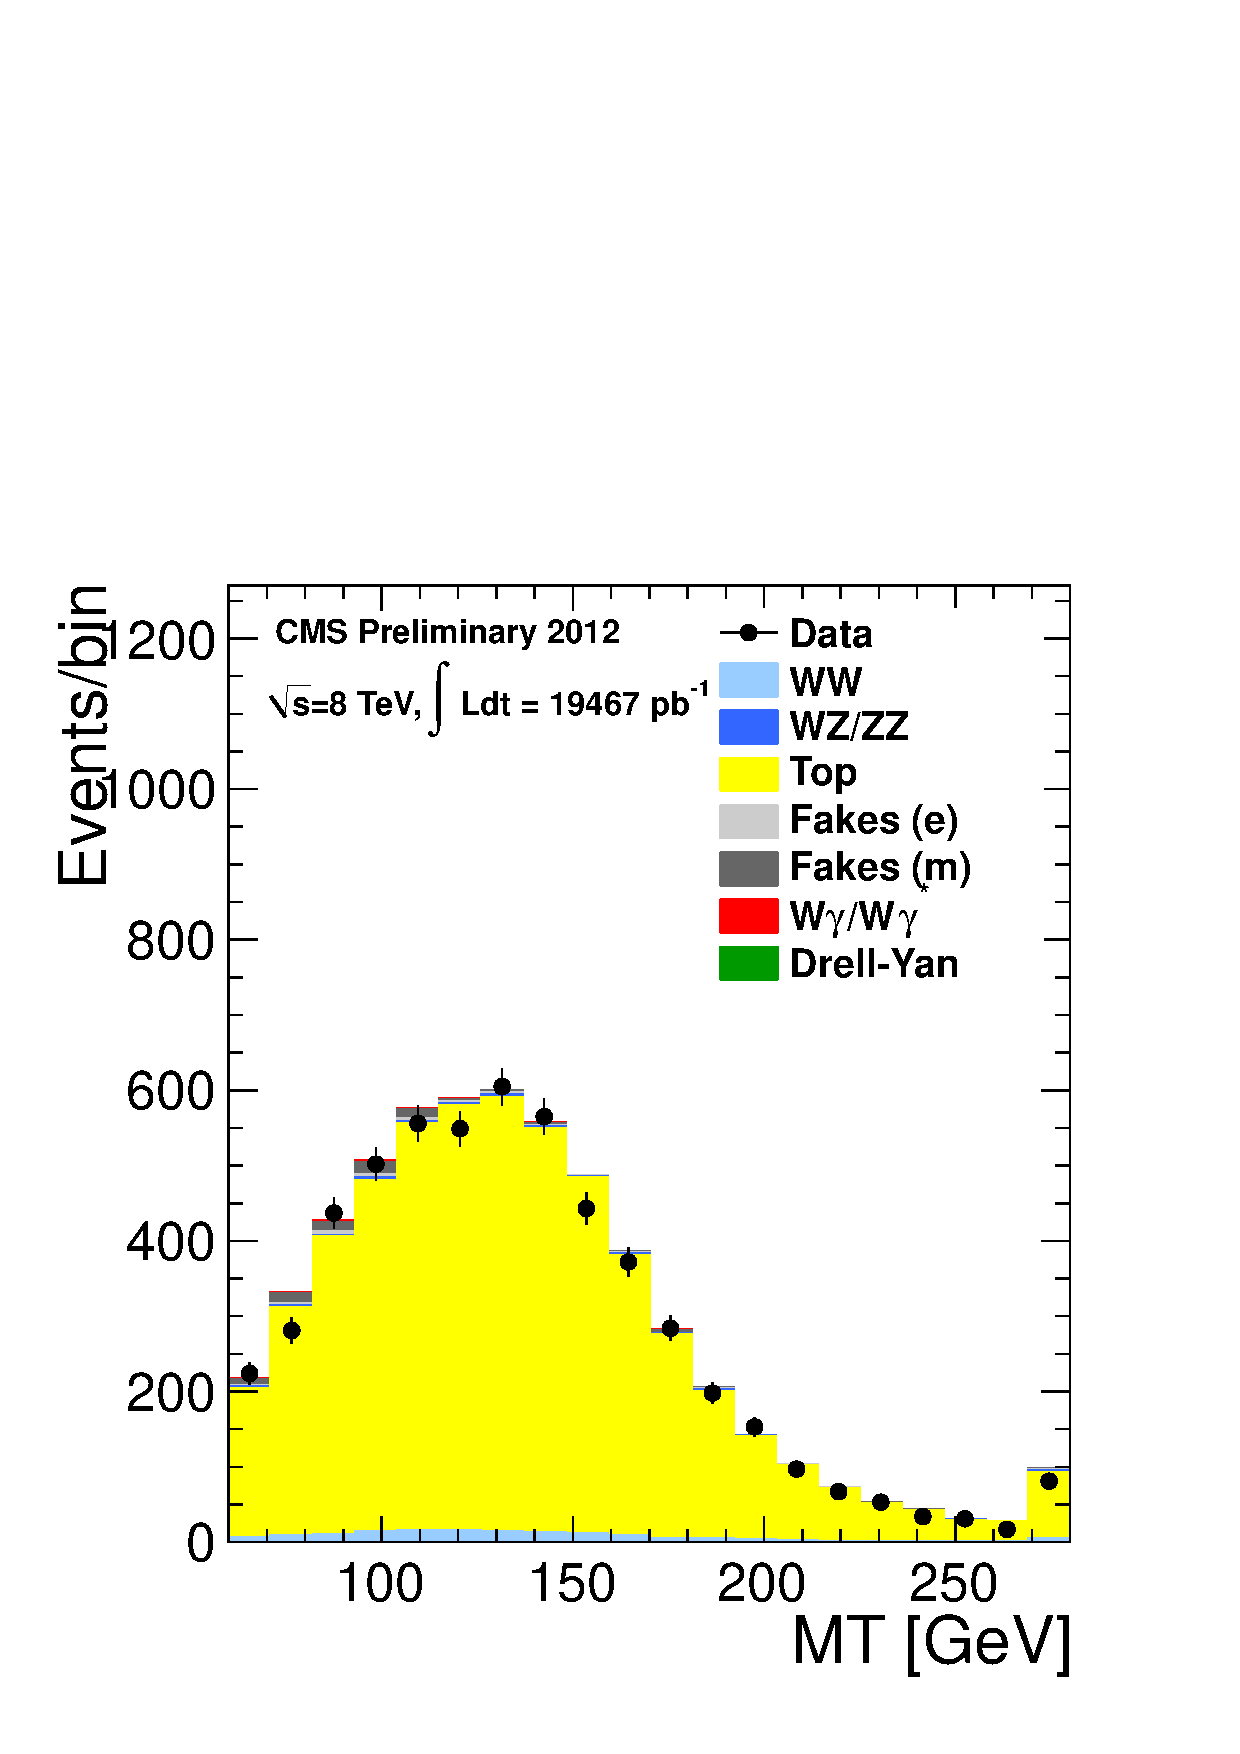
\includegraphics[width=.31\textwidth]{figures/hww_analysis16_0_ALL_of_1j_mt_toptag.pdf}
}\\

\caption{Kinematic distributions of events in the Top enriched background in the 1-Jet bin. We apply 
the WW selection inverting the Top veto requirements. }
\label{fig:toptagplots}
\end{figure}


